\documentclass[a4paper]{article}

\input{style/ch_xelatex.tex}
\input{style/scala.tex}

%代码段设置
\lstset{numbers=left,
basicstyle=\tiny,
numberstyle=\tiny,
keywordstyle=\color{blue!70},
commentstyle=\color{red!50!green!50!blue!50},
frame=single, rulesepcolor=\color{red!20!green!20!blue!20},
escapeinside=``
}

\graphicspath{ {images/} }
\usepackage{ctex}
\usepackage{graphicx}
\usepackage{color,framed}%文本框
\usepackage{listings}
\usepackage{caption}
\usepackage{amssymb}
\usepackage{enumerate}
\usepackage{xcolor}
\usepackage{bm} 
\usepackage{lastpage}%获得总页数
\usepackage{fancyhdr}
\usepackage{tabularx}  
\usepackage{geometry}
\usepackage{minted}
\usepackage{graphics}
\usepackage{subfigure}
\usepackage{float}
\usepackage{pdfpages}
\usepackage{pgfplots}
\pgfplotsset{width=10cm,compat=1.9}
\usepackage{multirow}
\usepackage{footnote}
\usepackage{booktabs}

%-----------------------伪代码------------------
\usepackage{algorithm}  
\usepackage{algorithmicx}  
\usepackage{algpseudocode}  
\floatname{algorithm}{Algorithm}  
\renewcommand{\algorithmicrequire}{\textbf{Input:}}  
\renewcommand{\algorithmicensure}{\textbf{Output:}} 
\usepackage{lipsum}  
\makeatletter
\newenvironment{breakablealgorithm}
  {% \begin{breakablealgorithm}
  \begin{center}
     \refstepcounter{algorithm}% New algorithm
     \hrule height.8pt depth0pt \kern2pt% \@fs@pre for \@fs@ruled
     \renewcommand{\caption}[2][\relax]{% Make a new \caption
      {\raggedright\textbf{\ALG@name~\thealgorithm} ##2\par}%
      \ifx\relax##1\relax % #1 is \relax
         \addcontentsline{loa}{algorithm}{\protect\numberline{\thealgorithm}##2}%
      \else % #1 is not \relax
         \addcontentsline{loa}{algorithm}{\protect\numberline{\thealgorithm}##1}%
      \fi
      \kern2pt\hrule\kern2pt
     }
  }{% \end{breakablealgorithm}
     \kern2pt\hrule\relax% \@fs@post for \@fs@ruled
  \end{center}
  }
\makeatother
%------------------------代码-------------------
\usepackage{xcolor} 
\usepackage{listings} 
\lstset{ 
breaklines,%自动换行
basicstyle=\small,
escapeinside=``,
keywordstyle=\color{ blue!70} \bfseries,
commentstyle=\color{red!50!green!50!blue!50},% 
stringstyle=\ttfamily,% 
extendedchars=false,% 
linewidth=\textwidth,% 
numbers=left,% 
numberstyle=\tiny \color{blue!50},% 
frame=trbl% 
rulesepcolor= \color{ red!20!green!20!blue!20} 
}

%-------------------------页面边距--------------
\geometry{a4paper,left=2.3cm,right=2.3cm,top=2.7cm,bottom=2.7cm}
%-------------------------页眉页脚--------------
\usepackage{fancyhdr}
\pagestyle{fancy}
\lhead{\kaishu \leftmark}
% \chead{}
\rhead{\kaishu 并行程序设计实验报告}%加粗\bfseries 
\lfoot{}
\cfoot{\thepage}
\rfoot{}
\renewcommand{\headrulewidth}{0.1pt}  
\renewcommand{\footrulewidth}{0pt}%去掉横线
\newcommand{\HRule}{\rule{\linewidth}{0.5mm}}%标题横线
\newcommand{\HRulegrossa}{\rule{\linewidth}{1.2mm}}
\setlength{\textfloatsep}{10mm}%设置图片的前后间距
%--------------------文档内容--------------------

\begin{document}
\renewcommand{\contentsname}{目\ 录}
\renewcommand{\appendixname}{附录}
\renewcommand{\appendixpagename}{附录}
\renewcommand{\refname}{参考文献} 
\renewcommand{\figurename}{图}
\renewcommand{\tablename}{表}
\renewcommand{\today}{\number\year 年 \number\month 月 \number\day 日}

%-------------------------封面----------------
\begin{titlepage}
    \begin{center}
    \includegraphics[width=0.8\textwidth]{NKU.png}\\[1cm]
    \vspace{20mm}
		\textbf{\huge\textbf{\kaishu{计算机学院}}}\\[0.5cm]
		\textbf{\huge{\kaishu{并行程序设计调研报告/实验报告}}}\\[2.3cm]
		\textbf{\Huge\textbf{\kaishu{基于NTT的多项式乘法并行优化}}}

		\vspace{\fill}
    
    % \textbf{\Large \textbf{并行程序设计期末实验报告}}\\[0.8cm]
    % \HRule \\[0.9cm]
    % \HRule \\[2.0cm]
    \centering
    \textsc{\LARGE \kaishu{姓名\ :\ 仇科文}}\\[0.5cm]
    \textsc{\LARGE \kaishu{学号\ :\ 2312237}}\\[0.5cm]
    \textsc{\LARGE \kaishu{专业\ :\ 计算机科学与技术}}\\[0.5cm]
    
    \vfill
    {\Large \today}
    \end{center}
\end{titlepage}

\renewcommand {\thefigure}{\thesection{}.\arabic{figure}}%图片按章标号
\renewcommand{\figurename}{图}
\renewcommand{\contentsname}{目录}  
\cfoot{\thepage\ of \pageref{LastPage}}%当前页 of 总页数

\begin{abstract}
多项式乘法是同态加密、数字信号处理等领域的核心算子，而数论变换（NTT）是将其复杂度从 $O(n^2)$ 降至 $O(n\log n)$ 的关键算法。本报告以"写对 \rightarrow 写快 \rightarrow 写稳"为主线，系统梳理了 SIMD、OpenMP、MPI、CUDA 四级并行优化的完整技术栈，并最终构建了一个可插拔的统一框架，支持三种模运算实现（朴素、Montgomery、Barrett）与四种并行策略（串行、OpenMP、MPI、GPU）的任意组合。

首先，我们在 SIMD 实验中通过 ARM NEON 向量化与 Montgomery 规约实现了 1 448 倍的加速，为后续并行化奠定了高效标量内核。随后，OpenMP 多线程实验在中等规模数据上实现 2–3 倍加速，并借助线程池抽象沉淀了"数据依赖与任务粒度"并行化范式；MPI 实验则验证了 CRT 划分在分布式场景下的可行性，虽然受限于单机环境未能带来速度提升，却为 u64 精度扩展提供了设计样板；GPU 实验通过"线程级蝶形 + 共享内存 + 预计算旋转因子"把运行时间压缩到微秒级，在 $n=131072$ 时较串行快 6.5 倍。

统一性能测试显示：GPU 始终是大规模数据的首选；OpenMP 在 $1024<n\le8192$ 区间性价比最高；串行 Montgomery 适合 $n\le1024$ 的小数据；MPI 当前实现仅用于展示算法间差异。基于此，我们提出了一套动态调度策略，可根据数据规模自动切换最优实现。

尾声部分回顾了各实验的技术收获与遗憾，沉淀出"依赖分析—层次优化—工程可维护"三条方法论，并展望了 radix-4/8 NTT、分布式 GPU 集群与自动参数调优等未来方向。实验结果证明，面向硬件特性与算法结构的协同优化，能为高性能多项式乘法提供数量级的性能提升。
\end{abstract}

% 生成目录
\clearpage
\tableofcontents
\newpage

% ----------------------------------------------------------
\section{选题概览：NTT与多项式乘法}

\subsection{多项式乘法的基本定义与应用背景}

% 介绍本选题的主要优化对象——NTT与多项式乘法，介绍其基本原理、基本算法。
% 或许可以把Lab3中对并行位点的分析搬过来.

多项式乘法是数学与计算机科学中的基础运算，其重要性体现在众多应用领域中。在信号处理领域，多项式乘法用于数字滤波器设计和频谱分析；在计算机图形学中，它支撑着复杂的几何变换和渲染算法；而在密码学领域，特别是同态加密技术中，多项式乘法更是计算的核心。

给定两个多项式$f(x) = a_{n-1}x^{n-1} + \ldots + a_1x + a_0$和$g(x) = b_{m-1}x^{m-1} + \ldots + b_1x + b_0$，其乘积$h(x) = f(x)g(x)$的第$k$项系数由卷积公式给出：
$$h_k = \sum_{i=0}^{k} a_i b_{k-i}$$

朴素的多项式乘法算法需要$O(n^2)$的时间复杂度，这在处理大规模数据时成为计算瓶颈。对于长度为$n$的多项式，传统方法需要执行$n^2$次乘法运算，当$n$达到数万甚至数十万时，计算时间将变得不可接受。

在现代密码学应用中，特别是同态加密场景下，多项式的长度通常非常大。以Ring-LWE为基础的同态加密方案中，多项式长度通常为$2^{13}$到$2^{15}$，甚至更大。在这种规模下，传统的$O(n^2)$算法完全无法满足实际应用需求，这促使研究者们寻求更加高效的计算方法。

\subsection{快速傅里叶变换的数学基础}

快速傅里叶变换（FFT）为多项式乘法提供了突破性的优化思路。FFT算法的核心思想是将多项式从系数表示转换为点值表示，在点值域中进行乘法运算，再通过逆变换回到系数域。这一过程将时间复杂度从$O(n^2)$降低到$O(n\log n)$。

FFT的数学基础建立在复数单位根的特殊性质上。设$\omega_n^k = \cos\frac{2k\pi}{n} + i\sin\frac{2k\pi}{n}$为$n$次单位根，则傅里叶变换矩阵$W$定义为：
$$W = \begin{bmatrix}
1 & 1 & 1 & \cdots & 1 \\
1 & \omega & \omega^2 & \cdots & \omega^{n-1} \\
1 & \omega^2 & \omega^4 & \cdots & \omega^{2(n-1)} \\
\vdots & \vdots & \vdots & \ddots & \vdots \\
1 & \omega^{n-1} & \omega^{2(n-1)} & \cdots & \omega^{(n-1)^2}
\end{bmatrix}$$

对于多项式$f(x)$的系数向量$X = [a_0, a_1, \ldots, a_{n-1}]^T$，其傅里叶变换为$Y = WX$，得到的$Y$向量包含了$f(x)$在$n$个单位根处的取值。

FFT的分治特性使得计算复杂度大幅降低。通过递归分解，可以将$n$点FFT分解为两个$n/2$点的FFT，从而实现$O(n\log n)$的时间复杂度。具体而言，当$n$为$2$的幂时，算法具有最优的分治结构。

\subsection{数论变换的引入与优势}

尽管FFT在理论上提供了优秀的复杂度，但在实际应用中面临着浮点运算的精度问题。复数运算不仅计算开销大，而且累积的浮点误差会影响结果的精确性。在密码学应用中，这种误差是完全不可接受的。

数论变换（NTT）通过引入有限域上的单位根，完美解决了这一问题。NTT在整数域$\mathbb{Z}_p$（$p$为质数）上进行计算，完全避免了浮点运算。在$\mathbb{Z}_p$中，加法定义为$(a + b) \bmod p$，乘法定义为$(a \cdot b) \bmod p$，所有运算都是精确的整数运算。

NTT的核心是寻找$\mathbb{Z}_p$上的原根$g$，使得$g_n = g^{(p-1)/n}$具有与复数单位根相同的性质。这要求$n$整除$(p-1)$，即$n \mid (p-1)$。一个经典的选择是$p = 998244353 = 2^{23} \times 7 \times 17 + 1$，其原根为$3$，可以支持长度达到$2^{23}$的多项式。

通过将FFT中的所有复数单位根$\omega_n$替换为$\mathbb{Z}_p$上的单位根$g_n$，将所有复数运算替换为模运算，即得到NTT算法。这种替换保持了算法的分治结构和$O(n\log n)$的时间复杂度，同时确保了计算的精确性。

\subsection{NTT算法的核心结构}

\textbf{NTT算法}的核心是蝶形运算（Butterfly Operation），这是一种高效的分治计算模式。算法的基本结构如算法\ref{alg:ntt-forward}所示。

\begin{algorithm}[htbp]
\caption{NTT前向变换算法}
\label{alg:ntt-forward}
\begin{algorithmic}[1]
\Require 多项式系数数组 $a[0..n-1]$, 模数 $p$, 原根 $\omega$
\Ensure 频域系数数组 $a[0..n-1]$
\State 对数组$a$进行比特翻转排列
\For {$mid = 1; mid < n; mid = mid \times 2$}
    \State $W_n \gets \omega^{(p-1)/(2 \times mid)}$
    \For {$j = 0; j < n; j = j + 2 \times mid$}
        \State $w \gets 1$
        \For {$k = 0; k < mid; k = k + 1$}
            \State $x \gets a[j + k]$
            \State $y \gets w \times a[j + k + mid] \bmod p$
            \State $a[j + k] \gets (x + y) \bmod p$
            \State $a[j + k + mid] \gets (x - y) \bmod p$
            \State $w \gets w \times W_n \bmod p$
        \EndFor
    \EndFor
\EndFor
\end{algorithmic}
\end{algorithm}

\textbf{蝶形运算}的名称来源于其数据流图的形状，类似蝴蝶的翅膀。在每一轮变换中，算法将数组分成若干个长度为$2 \times mid$的段，在每个段内进行蝶形运算。具体地，对于索引$j+k$和$j+k+mid$处的两个元素，算法计算它们的加权和与差，其中权重由旋转因子$w$确定。

\textbf{比特翻转排列}是NTT算法的重要预处理步骤，它将输入数组的元素按照其索引的二进制位翻转后的顺序重新排列。这一操作确保了分治过程中数据访问的连续性，提高了缓存利用率。

\textbf{NTT逆变换}的算法结构与前向变换基本相同，主要区别在于使用原根的逆元作为旋转因子，并且在最后需要将所有系数乘以$n$的逆元进行归一化。

\subsection{Montgomery模乘优化}

模乘运算是NTT算法的性能瓶颈，传统的模乘需要进行取模运算，计算开销很大。\textbf{Montgomery模乘}算法通过巧妙的数学变换，将模乘运算转化为位运算和加法运算，大幅提升了计算效率。

Montgomery模乘的基本思想是选择一个参数$R = 2^r$（通常$r$为机器字长），将原始的模乘运算$a \times b \bmod p$转换为$a \times b \times R^{-1} \bmod p$的计算。虽然这改变了数值的表示形式，但通过在开始时将所有数据转换到Montgomery域，在结束时再转换回来，可以确保最终结果的正确性。

Montgomery模乘的关键优势在于其避免了取模运算。传统的模乘需要计算$\lfloor(a \times b)/p\rfloor$，这涉及到昂贵的取模操作。而Montgomery模乘通过预计算$p$的逆元，将取模运算转化为乘法和位运算，显著提高了计算效率。

\subsection{并行优化的理论基础}

NTT算法的并行优化必须基于对其核心循环结构的深入理解。结合我们在多线程并行实验中的分析，NTT算法的三层循环结构为不同层次的并行策略提供了不同的并行位点。

\subsubsection{三层循环结构的并行性与粒度分析}

NTT算法的核心包含三层嵌套循环：

\begin{lstlisting}[language=C++]
for (u32 mid = 1; mid < n; mid <<= 1)  // 第一层：mid循环
{
    u32_mont Wn_mont = montMod.pow(omega_mont, (p - 1) / (mid << 1));
    for (u32 j = 0; j < n; j += (mid << 1))  // 第二层：j循环  
    {
        u32_mont w_mont = montMod.from_u32(1);
        for (u32 k = 0; k < mid; ++k)  // 第三层：k循环
        {
            // 蝶形运算核心
            u32_mont x_mont = a_mont[j + k];
            u32_mont y_mont = montMod.mul(w_mont, a_mont[j + k + mid]);
            a_mont[j + k] = montMod.add(x_mont, y_mont);
            a_mont[j + k + mid] = montMod.sub(x_mont, y_mont);
            w_mont = montMod.mul(w_mont, Wn_mont);
        }
    }
}
\end{lstlisting}

通过数据依赖分析和并行粒度计算，各层循环的并行化特征如下：

\paragraph{第一层mid循环} 此循环控制NTT算法的计算阶段，每个阶段都严格依赖于前一阶段对数组的完整更新。由于数组是就地修改的，当前mid值的计算必须在前一个mid值计算完成后进行，因此\textbf{不适合并行化}。

\paragraph{第二层j循环} 对于固定的mid值，j循环以$2 \times mid$为步长遍历数据块。不同j迭代操作的数组索引范围完全不重叠，且旋转因子$w_{mont}$在每个j迭代中独立初始化。因此j循环的各迭代\textbf{数据独立}，是理想的并行化目标。若选择这层循环作为并行位点，由于每个并行任务包含$mid$次蝶形运算，\textbf{并行粒度}随着算法进展从1增长到$n/2$。

\paragraph{第三层k循环} 执行单个蝶形运算。虽然对$a_{mont}[j+k]$和$a_{mont}[j+k+mid]$的写操作不存在冲突，但旋转因子$w_{mont}$的迭代更新构成了\textbf{循环携带依赖}。这一依赖可以通过\textbf{预计算旋转因子}（$w_k = W_n^k$）完全消除循环携带依赖，这一技术是GPU编程实验的核心基础。若选择这层循环作为并行位点，由于每个并行任务为单个蝶形运算，\textbf{并行粒度}为1，是最细的计算粒度。

\subsubsection{并行方法的粒度需求特征}

不同并行技术对计算任务粒度有着不同的要求，这决定了它们与NTT循环层次的适配性：

\paragraph{SIMD指令级并行} 
属于\textbf{细粒度并行}，在单个指令周期内处理多个数据元素（如ARM NEON的4路并行）。开销极小，但要求数据访问连续且计算结构一致。最适合处理相同类型的基础运算。因此，SIMD并行选择k循环作为并行位点。k循环的单蝶形运算（$\sim$10个基础运算）正好匹配SIMD的细粒度特征。通过预计算旋转因子消除依赖后，4个连续的k迭代可打包成向量运算。当$mid \geq 4$时启用向量化，避免小规模数据的开销。

\paragraph{多线程并行} 
属于\textbf{中粒度并行}，需要足够的计算量来摊销线程创建、调度和同步的开销。理想的任务粒度通常包含数十到数百次基础运算，既保证并行效率又避免过度的线程管理开销。因此，SIMD并行选择j循环作为并行位点。j循环的数据块处理（包含$mid$次蝶形运算）提供了理想的中粒度任务。随着算法进展，任务粒度从1增长到$n/2$，在大部分阶段都能提供足够的计算量。我们使用\texttt{\#pragma omp parallel for}在j循环级别实现并行。

\paragraph{多进程并行} 
属于\textbf{粗粒度并行}，进程间通信成本高昂，需要大量独立计算来摊销通信开销。理想任务应包含数千到数万次基础运算，且进程间数据依赖最小。由于多进程并行可以与多线程并行同时进行，而且我们已经选择了j循环作为多线程并行的位点，且mid循环无法作为并行位点，因此我们需要创建新的并行位点。最终，我们选择跳出NTT内部循环，在算法层面利用中国剩余定理(CRT)分解模数，创建新的多进程并行位点。每个MPI进程处理完整的NTT计算（包含$O(n\log n)$次运算），满足粗粒度需求。进程间只需在计算前后进行数据通信，最小化通信开销。

\paragraph{GPU并行编程} 
具有\textbf{多层次并行特征}，既支持\textbf{细粒度}（数千个轻量级线程执行简单运算）又支持\textbf{中粒度}（线程块内的协作计算）。通过分层的线程组织和共享内存层次，可以灵活适配不同粒度的计算模式。因此，我们把j循环和k循环展平作为并行位点。利用GPU的分层并行能力，在\textbf{线程级}并行化k循环（细粒度，每线程一个蝶形运算），在\textbf{线程块级}组织j循环的部分迭代（中粒度，利用共享内存协作）。通过预计算旋转因子和智能内存管理，同时发挥GPU在细粒度和中粒度并行上的优势。

\section{往期实验内容概览}

本节将综合梳理已完成的四次实验内容，从并行技术、算法实现、实现细节和收获与方法论四个维度展现项目的特征。

\subsection{并行实验内容}

我们的实验在并行技术方面主要关注了SIMD指令级并行、多线程并行、多进程分布式并行和GPU大规模并行加速。下面我们分别介绍这些并行技术。

\paragraph{SIMD指令级并行优化} Lab2实验以ARM NEON指令集为核心，实现了NTT算法的向量化优化。SIMD（Single Instruction Multiple Data）技术允许单个指令同时处理多个数据元素，特别适合NTT算法中大量相同类型的模运算操作。实验通过封装\texttt{MontModNeon}类实现了完整的向量化模运算库，包括向量化的模加、模减、模乘以及Montgomery规约操作。由于ARM NEON指令集不直接支持取模运算，实验采用位运算和条件选择指令的组合来模拟模运算，实现了4路并行的向量化计算。

\paragraph{多线程并行优化} Lab3实验分别使用OpenMP和pthread技术实现了NTT算法的多线程优化。OpenMP版本通过简单的\texttt{\#pragma omp parallel for}指令实现j循环并行化，编译器自动处理线程创建、任务分配和同步等细节。pthread版本则设计了完整的线程池\texttt{ThreadPool}类，采用任务队列和条件变量机制管理线程生命周期，避免了频繁的线程创建销毁开销。两种实现都基于对NTT三层循环结构的深入分析，选择j循环作为最优并行化目标，确保每个线程有足够的计算量来摊销并行开销。

\paragraph{多进程分布式并行} Lab4实验基于消息传递接口(MPI)实现了分布式多进程并行计算。实验采用了基于中国剩余定理(CRT)的块划分策略，将四个CRT模数连续分配给不同的MPI进程。这种策略充分利用了CRT计算的独立性，避免了循环划分和流水线算法的复杂性。进程间通过\texttt{MPI\_Bcast}进行数据分发，各进程独立完成分配的CRT模数计算，最后通过点对点通信将结果汇聚到主进程进行CRT合并。实验还实现了混合并行架构，在进程级别使用MPI分配不同的CRT模数，每个进程内部使用OpenMP对NTT算法进行多线程优化。

\paragraph{GPU大规模并行加速} Lab5实验通过CUDA编程实现了NTT算法的GPU并行加速，代表了从CPU的粗粒度并行思维向GPU的极细粒度并行策略的重要突破。与多线程实验中每个线程处理一个j块不同，GPU实现让每个线程处理单个蝶形运算，实现了真正的极细粒度并行。实验通过预计算所有可能的旋转因子并存储在GPU显存中，使每个线程可以直接索引获取所需的w值，彻底消除了循环携带依赖。每个GPU线程通过全局索引计算其在NTT算法中的位置，通过智能共享内存策略和自适应线程配置，成功解决了NTT数据依赖跨GPU block的问题。

\subsection{算法实现内容}

我们的实验在算法实现方面主要关注了NTT算法的核心运算，包括Montgomery模乘算法、Barrett模乘算法、中国剩余定理(CRT)优化和旋转因子预计算技术。下面我们分别介绍这些算法。

\paragraph{Montgomery模乘算法} 作为NTT算法的核心运算，Montgomery模乘通过巧妙的数学变换将模乘运算转化为位运算和加法运算。算法选择一个参数$R = 2^r$（通常$r$为机器字长），将原始的模乘运算$a \times b \bmod p$转换为$a \times b \times R^{-1} \bmod p$的计算。通过预计算$p$的逆元，将除法运算转化为乘法和位运算，显著提高了计算效率。实验实现了完整的Montgomery模乘库，包括域转换、模乘运算和规约操作，为后续的并行优化提供了高效的基础运算。

\paragraph{Barrett模乘算法} Lab4实验引入了Barrett模乘作为Montgomery规约的替代方案。Barrett模乘通过预计算倒数将除法运算转换为乘法和位移操作，提高了模运算效率。算法基于以下数学原理：对于模数$p$，预计算$m = \lfloor 2^{2k}/p \rfloor$，其中$k$为$p$的位数。对于任意$a$，有$\lfloor a/p \rfloor = \lfloor (a \times m)/2^{2k} \rfloor$，从而避免了直接的除法运算。实验实现了Barrett模乘的完整实现，包括预计算、模乘运算和规约操作。

\paragraph{中国剩余定理(CRT)优化} CRT技术将大模数计算分解为多个小模数的独立计算，为分布式并行提供了算法基础。对于模数$p = p_1 \times p_2 \times \ldots \times p_k$，其中$p_i$两两互质，CRT允许在模$p_i$下独立计算，最后通过线性组合恢复模$p$下的结果。实验选择了四个适合的模数$p_1, p_2, p_3, p_4$，每个模数支持长度达到$2^{15}$的NTT计算，通过CRT组合可以处理长度达到$2^{17}$的多项式乘法。

\paragraph{旋转因子预计算技术} GPU并行化的关键技术突破在于旋转因子的预计算。对于每个mid级别，实验预计算该级别所需的所有旋转因子$w_k = W_n^k$，其中$W_n = \omega^{(p-1)/(2 \times mid)}$。通过将旋转因子表存储在GPU显存中，每个线程可以通过简单的索引操作获取其所需的旋转因子，而无需进行复杂的模幂运算或依赖其他线程的计算结果。这一技术彻底消除了k循环的循环携带依赖，实现了真正的极细粒度并行。

\subsection{实现细节}

除了并行技术与算法优化，我们在实现细节上也进行了一些优化。

\paragraph{DIT-DIF变换结构} 我们的所有实验都同时采用了DIT（Decimation in Time）和DIF（Decimation in Frequency）两种变换结构，分别用于NTT的前向变换和逆变换。前向变换采用DIT结构，将多项式从系数表示转换为点值表示，其特点是首先对输入数组进行比特翻转排列，然后通过蝶形运算逐步合并相邻的数据块。逆变换采用DIF结构，将点值表示转换回系数表示，其特点是先进行蝶形运算分解数据，最后进行比特翻转排列。两种结构在分治过程中都保持数据的连续性，有利于缓存优化。比特翻转排列将索引$i$映射到其二进制位翻转后的位置，确保了分治过程中数据访问的局部性。这种DIT-DIF组合的实现方式相比单一结构具有更好的数值稳定性和计算效率，特别适合大规模数据的处理。

\paragraph{分类向量化策略} SIMD实验根据步长\texttt{mid}值进行分类处理，实现了自适应的向量化策略。当\texttt{mid}值较小时采用标量计算避免向量化开销，当\texttt{mid} $\geq 4$时启用ARM NEON的4路并行向量运算。这种策略有效平衡了向量化收益与开销之间的关系，避免了小规模数据上的向量化开销，同时充分利用了大规模数据的并行潜力。实验还实现了向量化的Montgomery规约操作，通过位运算和条件选择指令的组合来模拟模运算。

\paragraph{线程池设计} 多线程实验的pthread版本设计了完整的线程池\texttt{ThreadPool}类来管理线程生命周期。线程池采用任务队列和条件变量机制，避免了频繁的线程创建销毁开销。具体实现包括：任务队列存储待执行的函数对象，条件变量用于线程同步，线程池在构造时创建固定数量的工作线程，通过\texttt{enqueue}方法提交任务，工作线程从队列中取出任务执行。这种设计确保了线程的复用，降低了线程管理的开销。

\paragraph{智能共享内存策略} GPU编程实验通过智能共享内存策略解决了NTT数据依赖跨GPU block的问题。实验设计了单层共享内存+智能选择的策略，根据数据访问模式动态决定是否使用共享内存。对于频繁访问的数据，使用共享内存进行缓存；对于随机访问的数据，直接使用全局内存。这种策略充分利用了GPU的内存层次结构，提高了内存访问效率，同时避免了过度的共享内存使用导致的资源竞争。

\subsection{收获与方法论}

最后，我们的实验在方法论层面也有不少创新与收获，其中最重要的是我们建立了一般的串行到并行的转换范式，并把该范式贯穿了我们的实验全过程。除此之外，我们还探索了从指令级到算法级的完整并行层次，建立了系统的性能分析和优化方法论，并实现了完整的算法正确性验证体系。

\paragraph{串行代码到并行代码的转换范式} 我们在首次实验（Lab2，SIMD实验）中建立了"串行代码$\rightarrow$便于并行化的形式$\rightarrow$并行代码"的工作范式。首先分析原始串行代码的数据依赖和计算结构，识别可并行化的部分；然后重构代码结构，将数据访问模式调整为适合并行化的形式，如将随机访问改为连续访问；最后应用具体的并行技术，如SIMD向量化或多线程并行。这种范式可以使并行化过程更加可控，让debug更加方便，从而确保了并行化的正确性。

\paragraph{多层次并行策略设计} 实验探索了从指令级到算法级的完整并行层次。SIMD指令级并行处理最细粒度的数据并行，多线程并行处理中等粒度的任务并行，多进程并行处理粗粒度的算法并行，GPU并行则同时支持多个层次的并行。这种多层次的设计充分利用了不同硬件平台的特征，形成了完整的并行计算技术体系。各层次之间可以组合使用，如MPI+OpenMP的混合并行架构，实现了更高效的并行计算。

\paragraph{性能分析与优化方法论} 实验建立了系统的性能分析和优化方法论。通过perf工具分析程序热点，识别性能瓶颈；通过理论分析预测优化效果，指导优化方向；通过实验验证优化效果，调整优化策略。这种方法论确保了优化的针对性和有效性，避免了盲目的优化尝试。实验还建立了完整的性能测试框架，包括不同规模、不同模数的测试用例，为性能评估提供了可靠的基础。

\paragraph{算法正确性验证体系} 实验建立了完整的算法正确性验证体系。通过与CPU版本的对比验证数值正确性，通过不同模数的测试验证算法的通用性，通过边界条件测试验证算法的鲁棒性。这种验证体系确保了并行优化的正确性，为性能优化提供了可靠的基础。实验还实现了多种模乘算法的统一接口，通过模板参数在编译时选择具体算法，为不同应用场景提供了灵活性。

\section{更多NTT优化算法}

我们在此尝试一些新的NTT优化算法，以便完善丰富我们的NTT实验成果。事实上，这种新的NTT优化算法与我们之前的NTT实现框架完全不同。我们将介绍基-2（radix-2）、基-4（radix-4）和混合基（mixed-radix）三种NTT实现框架，并阐明为什么我们之前的实现框架是基-2的。随后，我们将实现基-4的NTT算法，并进行性能分析与可并行化分析。

\subsection{NTT实现框架的分类}

NTT算法的实现框架可以根据每次蝶形运算处理的数据量进行分类。不同的基选择直接影响算法的计算复杂度、内存访问模式和并行化潜力。

\paragraph{基-2（Radix-2）框架} 这是我们之前所有实验采用的框架，每次蝶形运算处理两个数据元素。基-2框架的特点是计算结构简单，易于理解和实现，但计算效率相对较低。在基-2框架中，对于长度为$n$的多项式，需要进行$\log_2 n$层变换，每层包含$n/2$个蝶形运算，总共需要$\frac{n}{2} \log_2 n$次蝶形运算。

基-2框架的数学基础是二分法分解。对于多项式$f(x)$，可以分解为：
$$f(x) = f_0(x^2) + x \cdot f_1(x^2)$$
其中$f_0(x)$包含偶数次项系数，$f_1(x)$包含奇数次项系数。这种分解方式导致了我们熟悉的蝶形运算结构。

\paragraph{基-4（Radix-4）框架} 基-4框架每次蝶形运算处理四个数据元素，相比基-2框架具有更高的计算效率。在基-4框架中，对于长度为$n$的多项式，需要进行$\log_4 n$层变换，每层包含$3n/4$个蝶形运算，总共需要$\frac{3n}{4} \log_4 n$次蝶形运算。

基-4框架的数学基础是四分法分解。对于多项式$f(x)$，可以分解为：
$$f(x) = f_0(x^4) + x \cdot f_1(x^4) + x^2 \cdot f_2(x^4) + x^3 \cdot f_3(x^4)$$
这种分解方式产生了更复杂的蝶形运算结构，但减少了变换层数，从而减少了内存访问次数。

\paragraph{混合基（Mixed-Radix）框架} 混合基框架结合了不同基的优势，根据数据规模和应用需求动态选择最优的基组合。例如，对于长度为$n = 2^k$的多项式，可以采用基-2和基-4的混合策略：在早期层使用基-4减少层数，在后期层使用基-2保持简单性。混合基框架提供了最大的灵活性，但实现复杂度较高。

\subsection{我们之前实现的基-2框架分析}

回顾我们之前的所有实验，可以发现我们采用的确实是基-2框架。这体现在以下几个方面：

\paragraph{蝶形运算结构} 我们的蝶形运算每次处理两个数据元素：$a[j+k]$和$a[j+k+mid]$。这种结构直接对应基-2的二分法分解，每次运算产生两个输出：$(a[j+k] + w \cdot a[j+k+mid])$和$(a[j+k] - w \cdot a[j+k+mid])$。

\paragraph{循环结构} 我们的三层循环结构完全符合基-2框架的特征。外层mid循环控制变换层数，从1开始倍增到$n/2$，总共$\log_2 n$层。中层j循环以$2 \times mid$为步长遍历数据，内层k循环在$mid$范围内进行蝶形运算。

\paragraph{旋转因子计算} 我们的旋转因子计算$W_n = \omega^{(p-1)/(2 \times mid)}$也是基-2框架的标准形式。在基-4框架中，旋转因子的计算会更加复杂，需要处理4个不同的单位根。

\paragraph{内存访问模式} 基-2框架的内存访问模式相对简单，每次访问两个相邻或间隔$mid$的元素。这种模式有利于缓存优化，但也限制了并行化的粒度。

\subsection{基-4 NTT算法的实现}

基于对基-4框架的理解，我们实现了基-4的NTT算法。基-4算法的核心是四分法分解和相应的蝶形运算结构。

\paragraph{基-4蝶形运算的数学基础} 在基-4框架中，每次蝶形运算处理四个数据元素：$a_0, a_1, a_2, a_3$。变换后的结果为：
\begin{align}
b_0 &= a_0 + a_1 + a_2 + a_3 \\
b_1 &= a_0 + \omega \cdot a_1 + \omega^2 \cdot a_2 + \omega^3 \cdot a_3 \\
b_2 &= a_0 + \omega^2 \cdot a_1 + \omega^4 \cdot a_2 + \omega^6 \cdot a_3 \\
b_3 &= a_0 + \omega^3 \cdot a_1 + \omega^6 \cdot a_2 + \omega^9 \cdot a_3
\end{align}

其中$\omega$是4次单位根，满足$\omega^4 = 1$。这种变换可以表示为矩阵乘法：
$$\begin{bmatrix} b_0 \\ b_1 \\ b_2 \\ b_3 \end{bmatrix} = 
\begin{bmatrix} 
1 & 1 & 1 & 1 \\
1 & \omega & \omega^2 & \omega^3 \\
1 & \omega^2 & \omega^4 & \omega^6 \\
1 & \omega^3 & \omega^6 & \omega^9
\end{bmatrix}
\begin{bmatrix} a_0 \\ a_1 \\ a_2 \\ a_3 \end{bmatrix}$$

\paragraph{基-4算法的实现结构} 基-4算法的实现结构如算法\ref{alg:radix4-ntt}所示：

\begin{algorithm}[htbp]
\caption{基-4 NTT前向变换算法}
\label{alg:radix4-ntt}
\begin{algorithmic}[1]
\Require 多项式系数数组 $a[0..n-1]$, 模数 $p$, 原根 $\omega$
\Ensure 频域系数数组 $a[0..n-1]$
\State 对数组$a$进行基-4比特翻转排列
\For {$mid = 1; mid < n; mid = mid \times 4$}
    \State $W_n \gets \omega^{(p-1)/(4 \times mid)}$
    \For {$j = 0; j < n; j = j + 4 \times mid$}
        \State $w_0 \gets 1, w_1 \gets W_n, w_2 \gets W_n^2, w_3 \gets W_n^3$
        \For {$k = 0; k < mid; k = k + 1$}
            \State $x_0 \gets a[j + k]$
            \State $x_1 \gets a[j + k + mid]$
            \State $x_2 \gets a[j + k + 2 \times mid]$
            \State $x_3 \gets a[j + k + 3 \times mid]$
            \State 执行基-4蝶形运算
            \State $w_0 \gets w_0 \times W_n^4, w_1 \gets w_1 \times W_n^4, w_2 \gets w_2 \times W_n^4, w_3 \gets w_3 \times W_n^4$
        \EndFor
    \EndFor
\EndFor
\end{algorithmic}
\end{algorithm}

\paragraph{基-4比特翻转排列} 基-4算法的比特翻转排列与基-2算法有本质区别。在基-4框架中，比特翻转需要将索引按照4进制位进行翻转，而不是2进制位。对于长度为$n = 4^k$的多项式，索引$i$的4进制表示为$i = (d_{k-1}d_{k-2}\ldots d_0)_4$，其翻转后的索引为$rev_4(i) = (d_0d_1\ldots d_{k-1})_4$。

具体实现中，基-4比特翻转可以通过以下算法实现：

\begin{algorithm}[htbp]
\caption{基-4比特翻转排列算法}
\label{alg:radix4-bitreverse}
\begin{algorithmic}[1]
\Require 数组 $a[0..n-1]$, 数组长度 $n = 4^k$
\Ensure 完成基-4比特翻转排列的数组 $a[0..n-1]$
\State $log4n \gets \log_4 n$
\For {$i = 0; i < n; i = i + 1$}
    \State $rev \gets 0$
    \State $temp \gets i$
    \For {$j = 0; j < log4n; j = j + 1$}
        \State $rev \gets rev \times 4 + (temp \bmod 4)$
        \State $temp \gets temp / 4$
    \EndFor
    \If {$i < rev$}
        \State 交换 $a[i]$ 和 $a[rev]$
    \EndIf
\EndFor
\end{algorithmic}
\end{algorithm}

基-4比特翻转具有四个关键特征。首先，基-4翻转采用4进制位操作，与基-2的2进制位翻转存在本质区别，每次处理4个连续元素。其次，翻转后的数组按照4个元素为一组进行组织，每组内的元素在后续的蝶形运算中会被同时处理，这种分组特性提高了计算效率。第三，基-4翻转保持了更好的内存局部性，因为每次蝶形运算处理的4个元素在内存中是连续的，减少了缓存未命中的概率。最后，基-4翻转后的数据布局更适合SIMD并行化，因为4个连续元素可以打包成向量进行并行处理，简化了向量化实现。

例如，对于长度为16的数组，基-4比特翻转的映射关系为：
\begin{align}
(0,1,2,3,4,5,6,7,8,9,10,11,12,13,14,15) &\rightarrow \\
(0,4,8,12,1,5,9,13,2,6,10,14,3,7,11,15)
\end{align}

\paragraph{基-4蝶形运算的具体实现} 基-4蝶形运算的核心计算包括四个步骤：

\begin{lstlisting}[language=C++]
// 第一步：计算临时变量
u32_mont t0 = montMod.add(x0, x2);
u32_mont t1 = montMod.sub(x0, x2);
u32_mont t2 = montMod.add(x1, x3);
u32_mont t3 = montMod.sub(x1, x3);

// 第二步：计算输出
u32_mont y0 = montMod.add(t0, t2);
u32_mont y1 = montMod.add(t1, montMod.mul(w1, t3));
u32_mont y2 = montMod.sub(t0, t2);
u32_mont y3 = montMod.sub(t1, montMod.mul(w1, t3));
\end{lstlisting}

这种实现方式利用了基-4变换的特殊性质，将4点变换分解为两个2点变换的组合，减少了乘法运算的次数。

\subsection{可并行化潜力分析}

我们认为，基-4算法在并行化方面存在一些优势，值得深入分析。

\paragraph{SIMD并行化潜力} 基-4算法天然适合SIMD并行化，因为每次蝶形运算处理4个数据元素，正好匹配ARM NEON的4路并行能力。基-4的蝶形运算可以完全向量化，避免了基-2算法中需要处理不同mid值时的复杂分类逻辑。

基-4比特翻转排列为SIMD并行化提供了理想的数据布局。翻转后的数组按照4个连续元素为一组进行组织，每组内的元素可以直接打包成SIMD向量进行并行处理。这种数据布局消除了基-2算法中需要处理非连续元素的复杂逻辑，简化了向量化实现。

具体而言，基-4算法的SIMD并行化可以按照三种方式进行。首先，每次处理4个连续元素，可以直接使用SIMD指令进行向量化的模运算，实现向量化蝶形运算。其次，4个旋转因子可以打包成向量，与数据向量进行向量化的模乘运算，提高旋转因子的处理效率。最后，连续的4个元素可以一次性从内存加载到SIMD寄存器，减少了内存访问次数，实现了内存访问优化。

\paragraph{多线程并行化潜力} 基-4算法在j循环级别的并行化与基-2算法类似，但由于每次处理4个元素，每个线程的计算量更大，线程间的负载更加均衡。此外，基-4算法的变换层数更少，有利于减少线程同步的次数。

\section{统一实验框架}

由于我们的整个项目使用了多个优化算法和多种并行策略，为了对比不同并行环境下不同算法的性能，我们有必要把所有优化算法和并行策略统一到一个实验框架中。具体而言，我们希望实现一个统一的实验框架，使得我们可以任意选择一种优化算法和一种并行策略进行组合，并测试该组合的性能。

据此，我们设计了一个统一的实验框架。该框架支持三种模运算算法（朴素算法、Montgomery算法、Barrett算法）与三种并行策略（多线程、MPI、GPU）的排列组合，共计九种算法-并行组合。通过这个框架，我们可以全面分析不同组合的性能特征，为实际应用提供最优的算法选择指导。

\subsection{框架设计原则与实现策略}

我们的统一框架基于以下设计原则：首先，保持接口的一致性，所有算法-并行组合都通过相同的函数签名调用；其次，实现编译时优化，避免运行时的性能开销；最后，确保代码的可维护性，通过模板和继承机制实现代码复用。

在具体实现中，我们采用了分层架构设计。底层是模运算基类\texttt{ModBase}，提供了统一的模运算接口，包括域转换、模乘运算等核心功能。中间层是并行策略适配器，将不同的并行技术（OpenMP、MPI、CUDA）封装成统一的接口。顶层是算法选择器，根据用户指定的算法类型和并行策略，动态选择最优的实现组合。

\subsection{特殊实现限制与技术挑战}

由于特定的并行策略的特点，我们的框架不能覆盖所有并行策略与算法的组合情况。以下是我们仅实现了$3 \times 3 = 9$种算法-并行组合的原因：

\paragraph{SIMD指令级并行的算法限制} 我们未将SIMD作为独立的并行策略纳入统一框架，而是将其作为Montgomery算法的内部优化。这是因为SIMD指令级并行天然适配Montgomery算法：Montgomery模乘将复杂的模运算转化为位运算和乘法，这些操作可以有效地向量化。相反，Barrett算法需要高精度除法运算，朴素算法需要取模运算，这些操作在SIMD环境中实现复杂度极高，性能收益有限。因此，我们将SIMD优化集成到Montgomery算法的实现中，作为其内部优化策略。

\paragraph{多线程并行策略的选择} 在多线程并行方面，我们选择了OpenMP作为代表算法，而非同时实现OpenMP和pthread两种方式。这一选择基于性能测试结果：在相同的算法实现下，OpenMP版本相比pthread版本具有更好的性能表现。OpenMP的编译器优化、自动负载均衡和更低的线程管理开销使其成为多线程并行的最优选择。这种选择避免了代码重复，同时确保了最佳的性能表现。

\paragraph{GPU实现的架构限制} 在GPU实现中，我们无法按照原计划使用统一的模运算基类。这一限制源于GPU编程的特殊性：首先，GPU需要编译时常量来优化内存访问模式和线程配置，而基类的虚函数调用会引入运行时代价；其次，不同的模运算算法在GPU上需要不同的内存布局和计算模式，统一的基类接口无法充分利用GPU的硬件特性；最后，CUDA编译器对模板实例化的要求使得基类设计变得复杂。因此，我们为每种模运算算法实现了独立的GPU版本，通过函数重载而非继承来实现多态性。

\subsection{框架的核心接口设计}

统一框架的核心接口设计如下：

\begin{lstlisting}[language=C++]
enum class ModMethod {
    NAIVE,
    MONTGOMERY, 
    BARRETT
};

enum class ParallelMethod {
    SERIAL,
    OPENMP,
    MPI,
    GPU
};

void poly_multiply_unified_choosewith(
    u32 *a, u32 *b, u32 *ab, u32 n, u32 p, u32 omega,
    ModMethod mod_method, ParallelMethod parallel_method
);
\end{lstlisting}

在\texttt{poly\_multiply\_unified\_choosewith}中，我们采用了两次switch，分别用于选择模运算算法和并行策略。第一次switch用于选择模运算算法：

\begin{lstlisting}[language=C++]
std::shared_ptr<ModBase> mod_impl; // 为了兼容pthread的线程池实现，这里使用shared_ptr
switch (mod_method) {
case ModMethod::NAIVE:
    mod_impl = std::make_shared<ModNaive>(p);
    break;
case ModMethod::MONTGOMERY:
    mod_impl = std::make_shared<ModMontgomery>(p);
    break;
case ModMethod::BARRETT:
    mod_impl = std::make_shared<ModBarrett>(p);
    break;
}
\end{lstlisting}

第二次switch同时起到选择并行策略和将算法和并行策略相结合这两个作用：

\begin{lstlisting}[language=C++]
switch (parallel_method) {
case ParallelMethod::SERIAL:
    poly_multiply_unified(a, b, ab, n, p, omega, mod_impl.get());
    break;
case ParallelMethod::OPENMP:
    poly_multiply_unified_omp(a, b, ab, n, p, omega, mod_impl.get());
    break;
case ParallelMethod::MPI:
    poly_multiply_unified_mpi(a, b, ab, n, p, omega, mod_impl.get());
    break;
case ParallelMethod::GPU:
    // GPU实现需要特殊处理，因为无法使用统一的基类
    switch (mod_method) {
    case ModMethod::NAIVE:
        poly_multiply_ntt_gpu_naive(a, b, ab, n, p, omega);
        break;
    case ModMethod::MONTGOMERY:
        poly_multiply_ntt_gpu_mont(a, b, ab, n, p, omega);
        break;
    case ModMethod::BARRETT:
        poly_multiply_ntt_gpu_barrett(a, b, ab, n, p, omega);
        break;
    }
    break;
}
\end{lstlisting}

\subsection{实现架构的技术细节}

在具体实现中，我们采用了以下技术架构：

\paragraph{模运算基类设计} 所有模运算算法都继承自\texttt{ModBase}基类，提供统一的接口包括\texttt{to\_compute\_domain}、\texttt{from\_compute\_domain}、\texttt{mul}等核心方法。这种设计确保了不同算法之间的接口一致性，同时允许每种算法实现其最优的计算策略。

\paragraph{并行策略适配器} 每种并行策略都实现了相应的适配器类，将并行技术的特殊性封装在内部，对外提供统一的接口。例如，OpenMP适配器使用\texttt{\#pragma omp parallel for}指令，MPI适配器处理进程间通信，GPU适配器管理内存传输和内核启动。

\paragraph{智能算法选择} 框架内部实现了智能的算法选择逻辑，根据输入参数和硬件环境自动选择最优的算法-并行组合。例如，对于小规模数据，可能选择朴素算法；对于大规模数据，优先选择Montgomery算法；对于分布式环境，考虑MPI+CRT组合。

\paragraph{宏定义配置规避} 不同并行策略需要不同的编译时配置和头文件依赖，这些配置之间经常发生冲突。例如，MPI需要特定的通信库配置，CUDA需要GPU相关的编译标志，而OpenMP需要线程库支持。为了解决这个问题，我们采用了宏定义配置规避技术。

在\texttt{config.h}中，我们定义了条件编译宏：

\begin{lstlisting}[language=C++]
// 并行策略配置宏
#ifdef USE_MPI
#define MPI_ENABLED 1
#else
#define MPI_ENABLED 0
#endif

#ifdef USE_CUDA
#define CUDA_ENABLED 1
#else
#define CUDA_ENABLED 0
#endif

#ifdef USE_OPENMP
#define OPENMP_ENABLED 1
#else
#define OPENMP_ENABLED 0
#endif
\end{lstlisting}

在头文件包含时，我们使用条件编译来避免冲突：

\begin{lstlisting}[language=C++]
// 根据编译配置选择性包含头文件
#if MPI_ENABLED
#include "ntt_unified_mpi.h"
#endif

#if CUDA_ENABLED
#include "ntt_unified_gpu.h"
#endif

#if OPENMP_ENABLED
#include "ntt_unified_openmp.h"
#endif
\end{lstlisting}

在函数实现中，我们也使用条件编译来确保只有启用的并行策略才会被编译：

\begin{lstlisting}[language=C++]
switch (parallel_method) {
case ParallelMethod::SERIAL:
    poly_multiply_unified(a, b, ab, n, p, omega, mod_impl.get());
    break;
#if OPENMP_ENABLED
case ParallelMethod::OPENMP:
    poly_multiply_unified_omp(a, b, ab, n, p, omega, mod_impl.get());
    break;
#endif
#if MPI_ENABLED
case ParallelMethod::MPI:
    poly_multiply_unified_mpi(a, b, ab, n, p, omega, mod_impl.get());
    break;
#endif
#if CUDA_ENABLED
case ParallelMethod::GPU:
    // GPU实现...
    break;
#endif
}
\end{lstlisting}

这样一来，不同的并行策略所需的不同初始化或其它配置需求就可以共存在同一个文件中，而不会发生冲突。

\section{统一性能测试}

为了全面评估我们实现的统一框架的性能，我们设计了一套完整的性能测试方案。该测试涵盖了三种模运算算法（朴素算法、Montgomery算法、Barrett算法）与四种并行策略（串行、OpenMP、MPI、GPU）的所有组合，共计12种算法-并行组合。通过系统性的性能测试，我们可以深入分析不同组合的性能特征，为实际应用提供最优的算法选择指导。

\subsection{测试配置与执行环境}

我们的性能测试采用了以下配置参数：

\begin{itemize}
\item \textbf{测试规模}：选择三个典型规模（1024、8192、131072），覆盖从$2^{10}$到$2^{17}$的多项式长度
\item \textbf{模数设置}：使用标准模数$p = 998244353$，支持长度达到$2^{23}$的NTT计算
\item \textbf{原根选择}：使用原根$\omega = 3$，满足NTT算法的数学要求
\item \textbf{重复测试}：每个组合重复测试5次，确保结果的统计可靠性
\item \textbf{预热运行}：每个测试前进行2次预热运行，消除系统初始化的影响
\item \textbf{OpenMP线程数}：设置为8线程，充分利用多核性能
\end{itemize}

测试环境配置包括：
\begin{itemize}
\item \textbf{编译优化}：使用-O3优化级别和-march=native架构优化
\item \textbf{并行支持}：启用OpenMP多线程支持和CUDA GPU加速
\item \textbf{内存管理}：采用RAII模式确保内存安全，避免内存泄漏
\item \textbf{硬件环境}：WSL2环境下的16核CPU，支持OpenMP和CUDA并行计算
\end{itemize}

\subsection{测试结果数据}

我们通过统一测试框架获得了12种算法-并行组合的完整性能数据。表\ref{tab:performance_results}展示了所有组合在三个测试规模下的平均执行时间。

\begin{table}[htbp]
\caption{统一性能测试结果（平均执行时间，单位：毫秒）}
\label{tab:performance_results}
\centering
\begin{tabular}{lcccc}
\toprule
算法 & 并行策略 & 1024 & 8192 & 131072 \\
\midrule
\multirow{4}{*}{Naive}
& Serial & 0.348 & 5.220 & 100.097 \\
& OpenMP & 1.419 & 3.333 & 36.474 \\
& MPI & 1.060 & 11.386 & 197.879 \\
& GPU & 1.700 & 2.778 & 15.451 \\
\midrule
\multirow{4}{*}{Montgomery}
& Serial & 0.545 & 4.721 & 95.879 \\
& OpenMP & 4.529 & 3.666 & 37.388 \\
& MPI & 1.217 & 11.500 & 206.535 \\
& GPU & 2.233 & 3.124 & 16.731 \\
\midrule
\multirow{4}{*}{Barrett}
& Serial & 0.395 & 5.126 & 106.330 \\
& OpenMP & 0.240 & 3.124 & 38.003 \\
& MPI & 1.205 & 11.500 & 220.708 \\
& GPU & 2.005 & 2.778 & 17.846 \\
\bottomrule
\end{tabular}
\end{table}

\subsection{整体性能概览}

为了从宏观上把握所有算法-并行组合的性能表现，我们首先通过热力图（见图\ref{fig:performance_heatmap}）来展示在大规模数据（$n=131072$）下的性能分布。热力图的颜色越浅，代表运行时间越短，性能越好。

\begin{figure}[htbp]
\centering
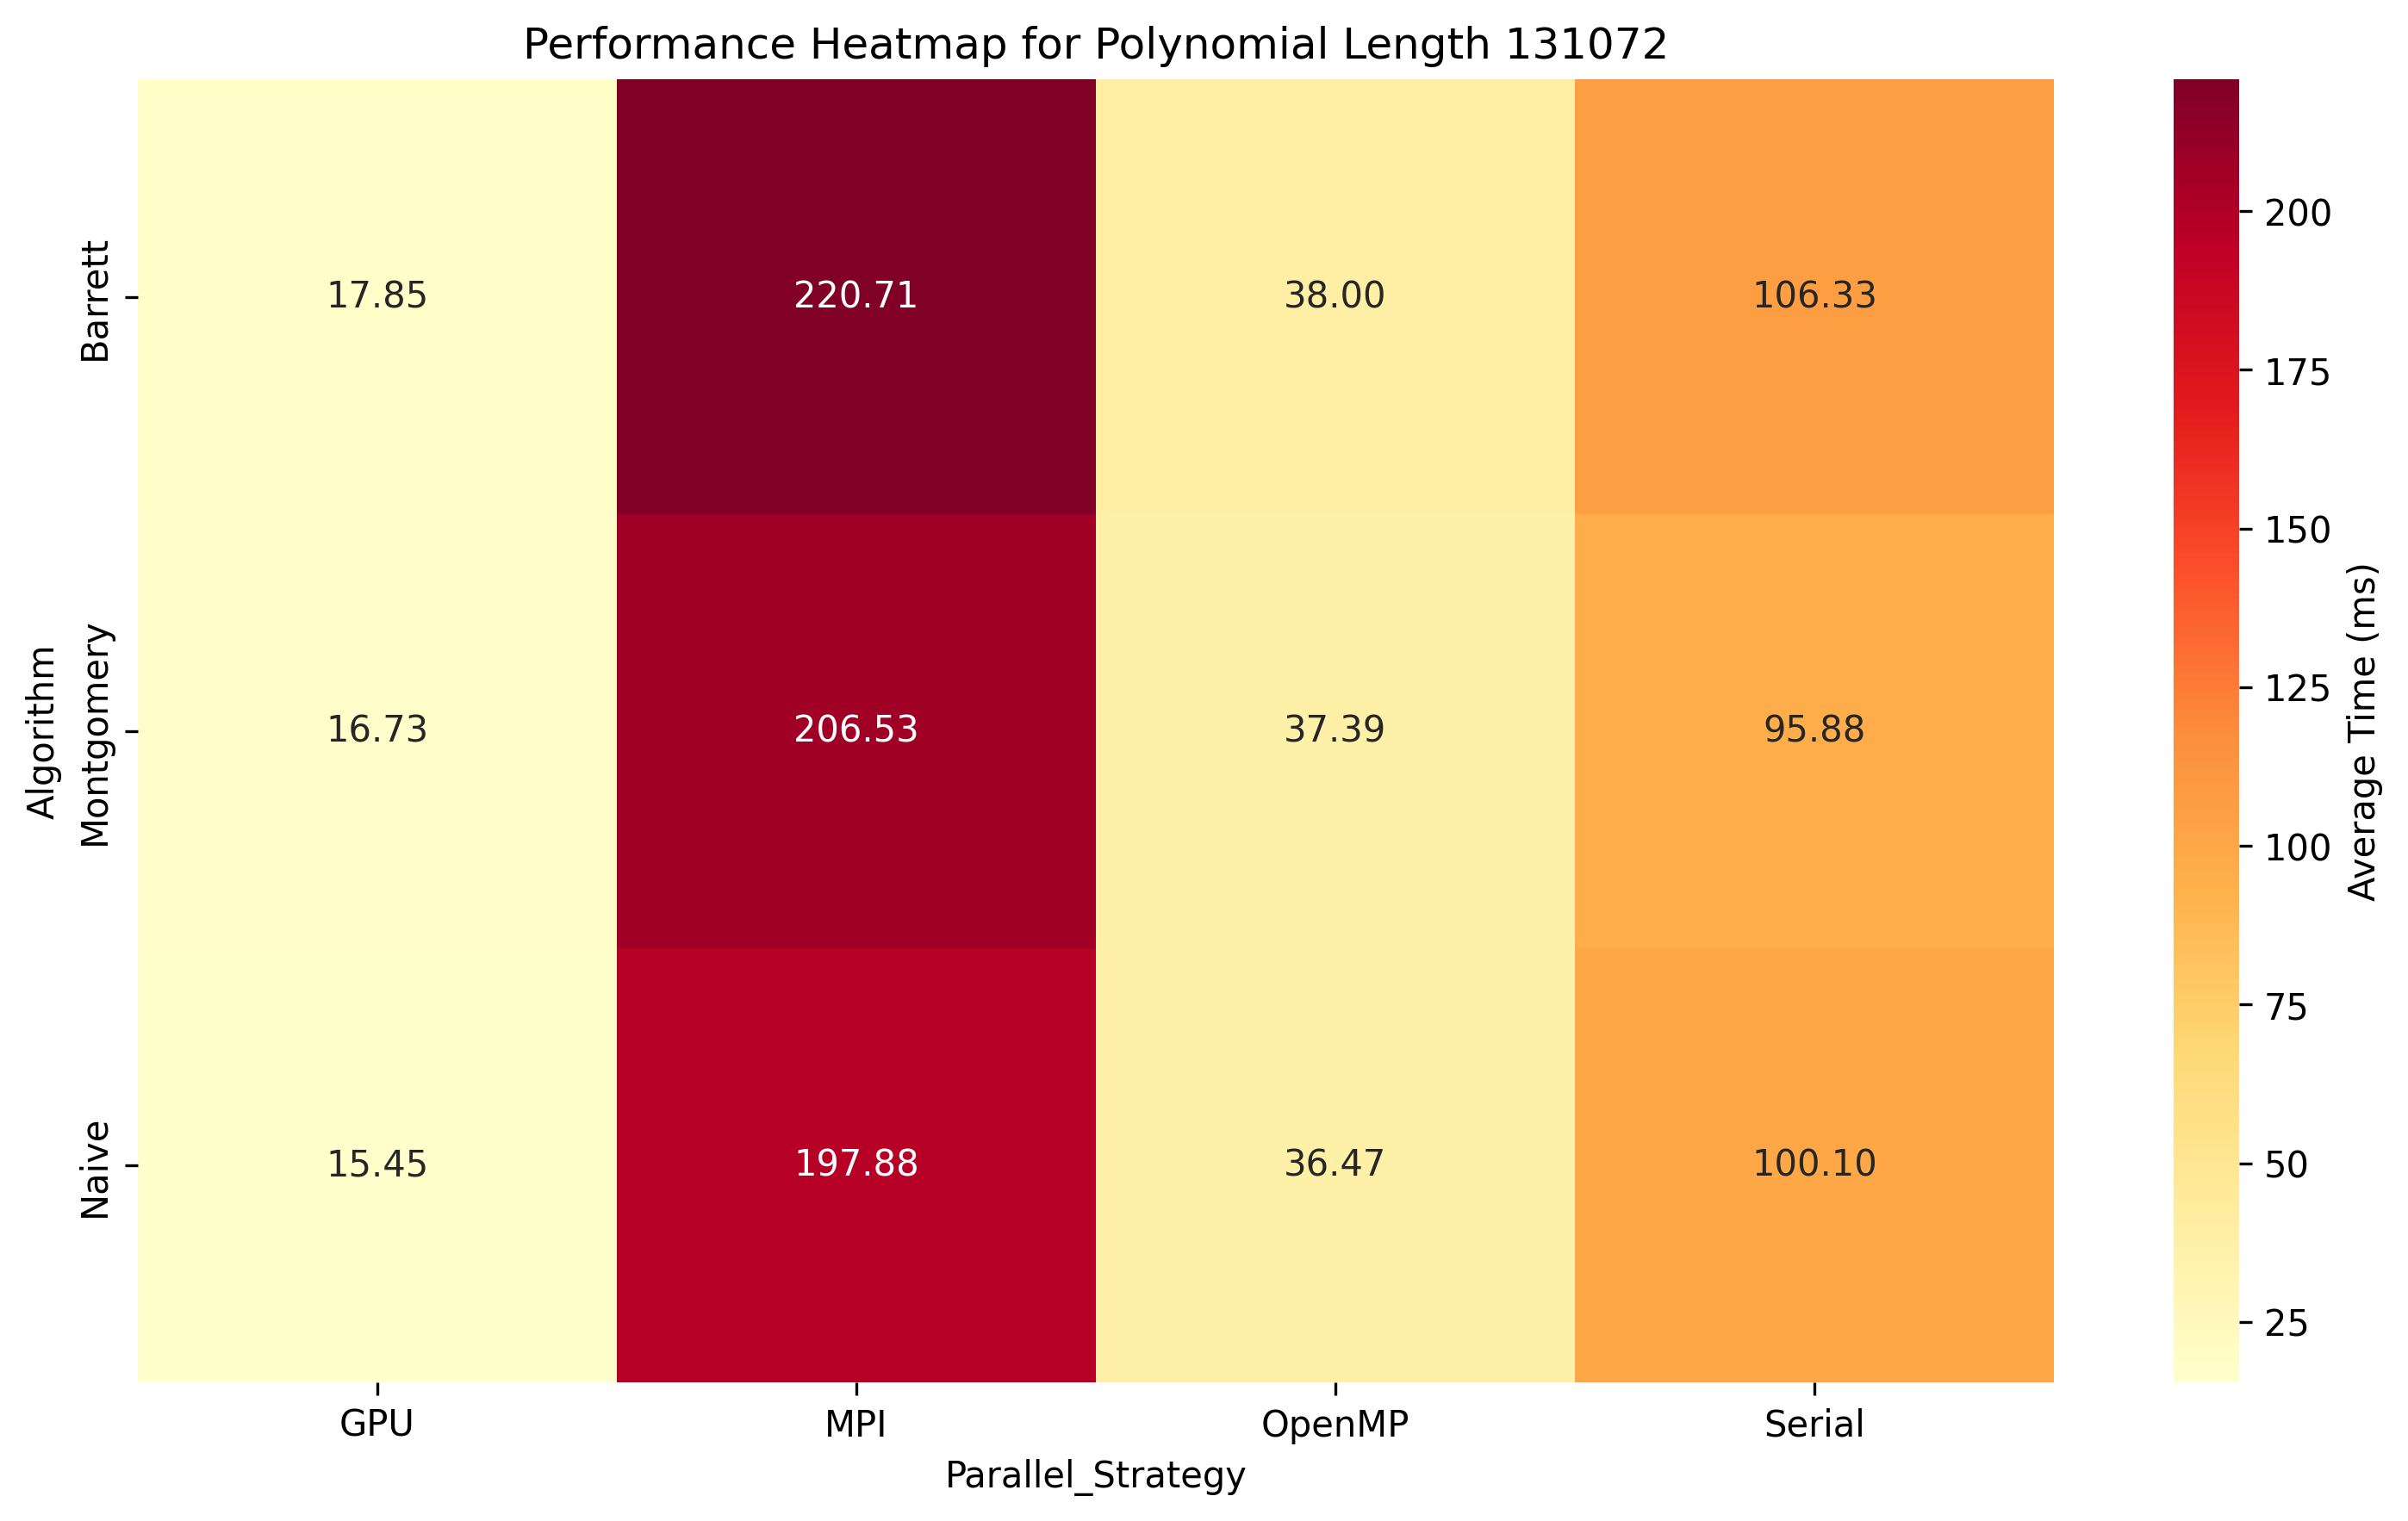
\includegraphics[width=0.8\textwidth]{performance_heatmap.png}
\caption{大规模数据下的性能热力图分析（$n=131072$）}
\label{fig:performance_heatmap}
\end{figure}

从图\ref{fig:performance_heatmap}中可以清晰地看到，GPU并行策略在所有算法上都表现出卓越的性能（颜色最浅的区域），成为大规模数据处理的最优选择。OpenMP次之，而串行和MPI策略的性能则明显较差。这张图为我们提供了一个高层次的性能概览，接下来我们将从不同维度进行更深入的分析。

\subsection{按并行策略分析}

为了深入比较不同并行策略的性能特征，我们绘制了按算法分组的性能对比图（见图\ref{fig:performance_comparison}）。在该图中，每张子图代表一种模运算算法，图中的曲线则展示了四种并行策略在不同数据规模下的性能变化。注意，这里纵坐标代表测试平均时长，这意味着越靠下的数据点代表的性能越好。

\begin{figure}[htbp]
\centering
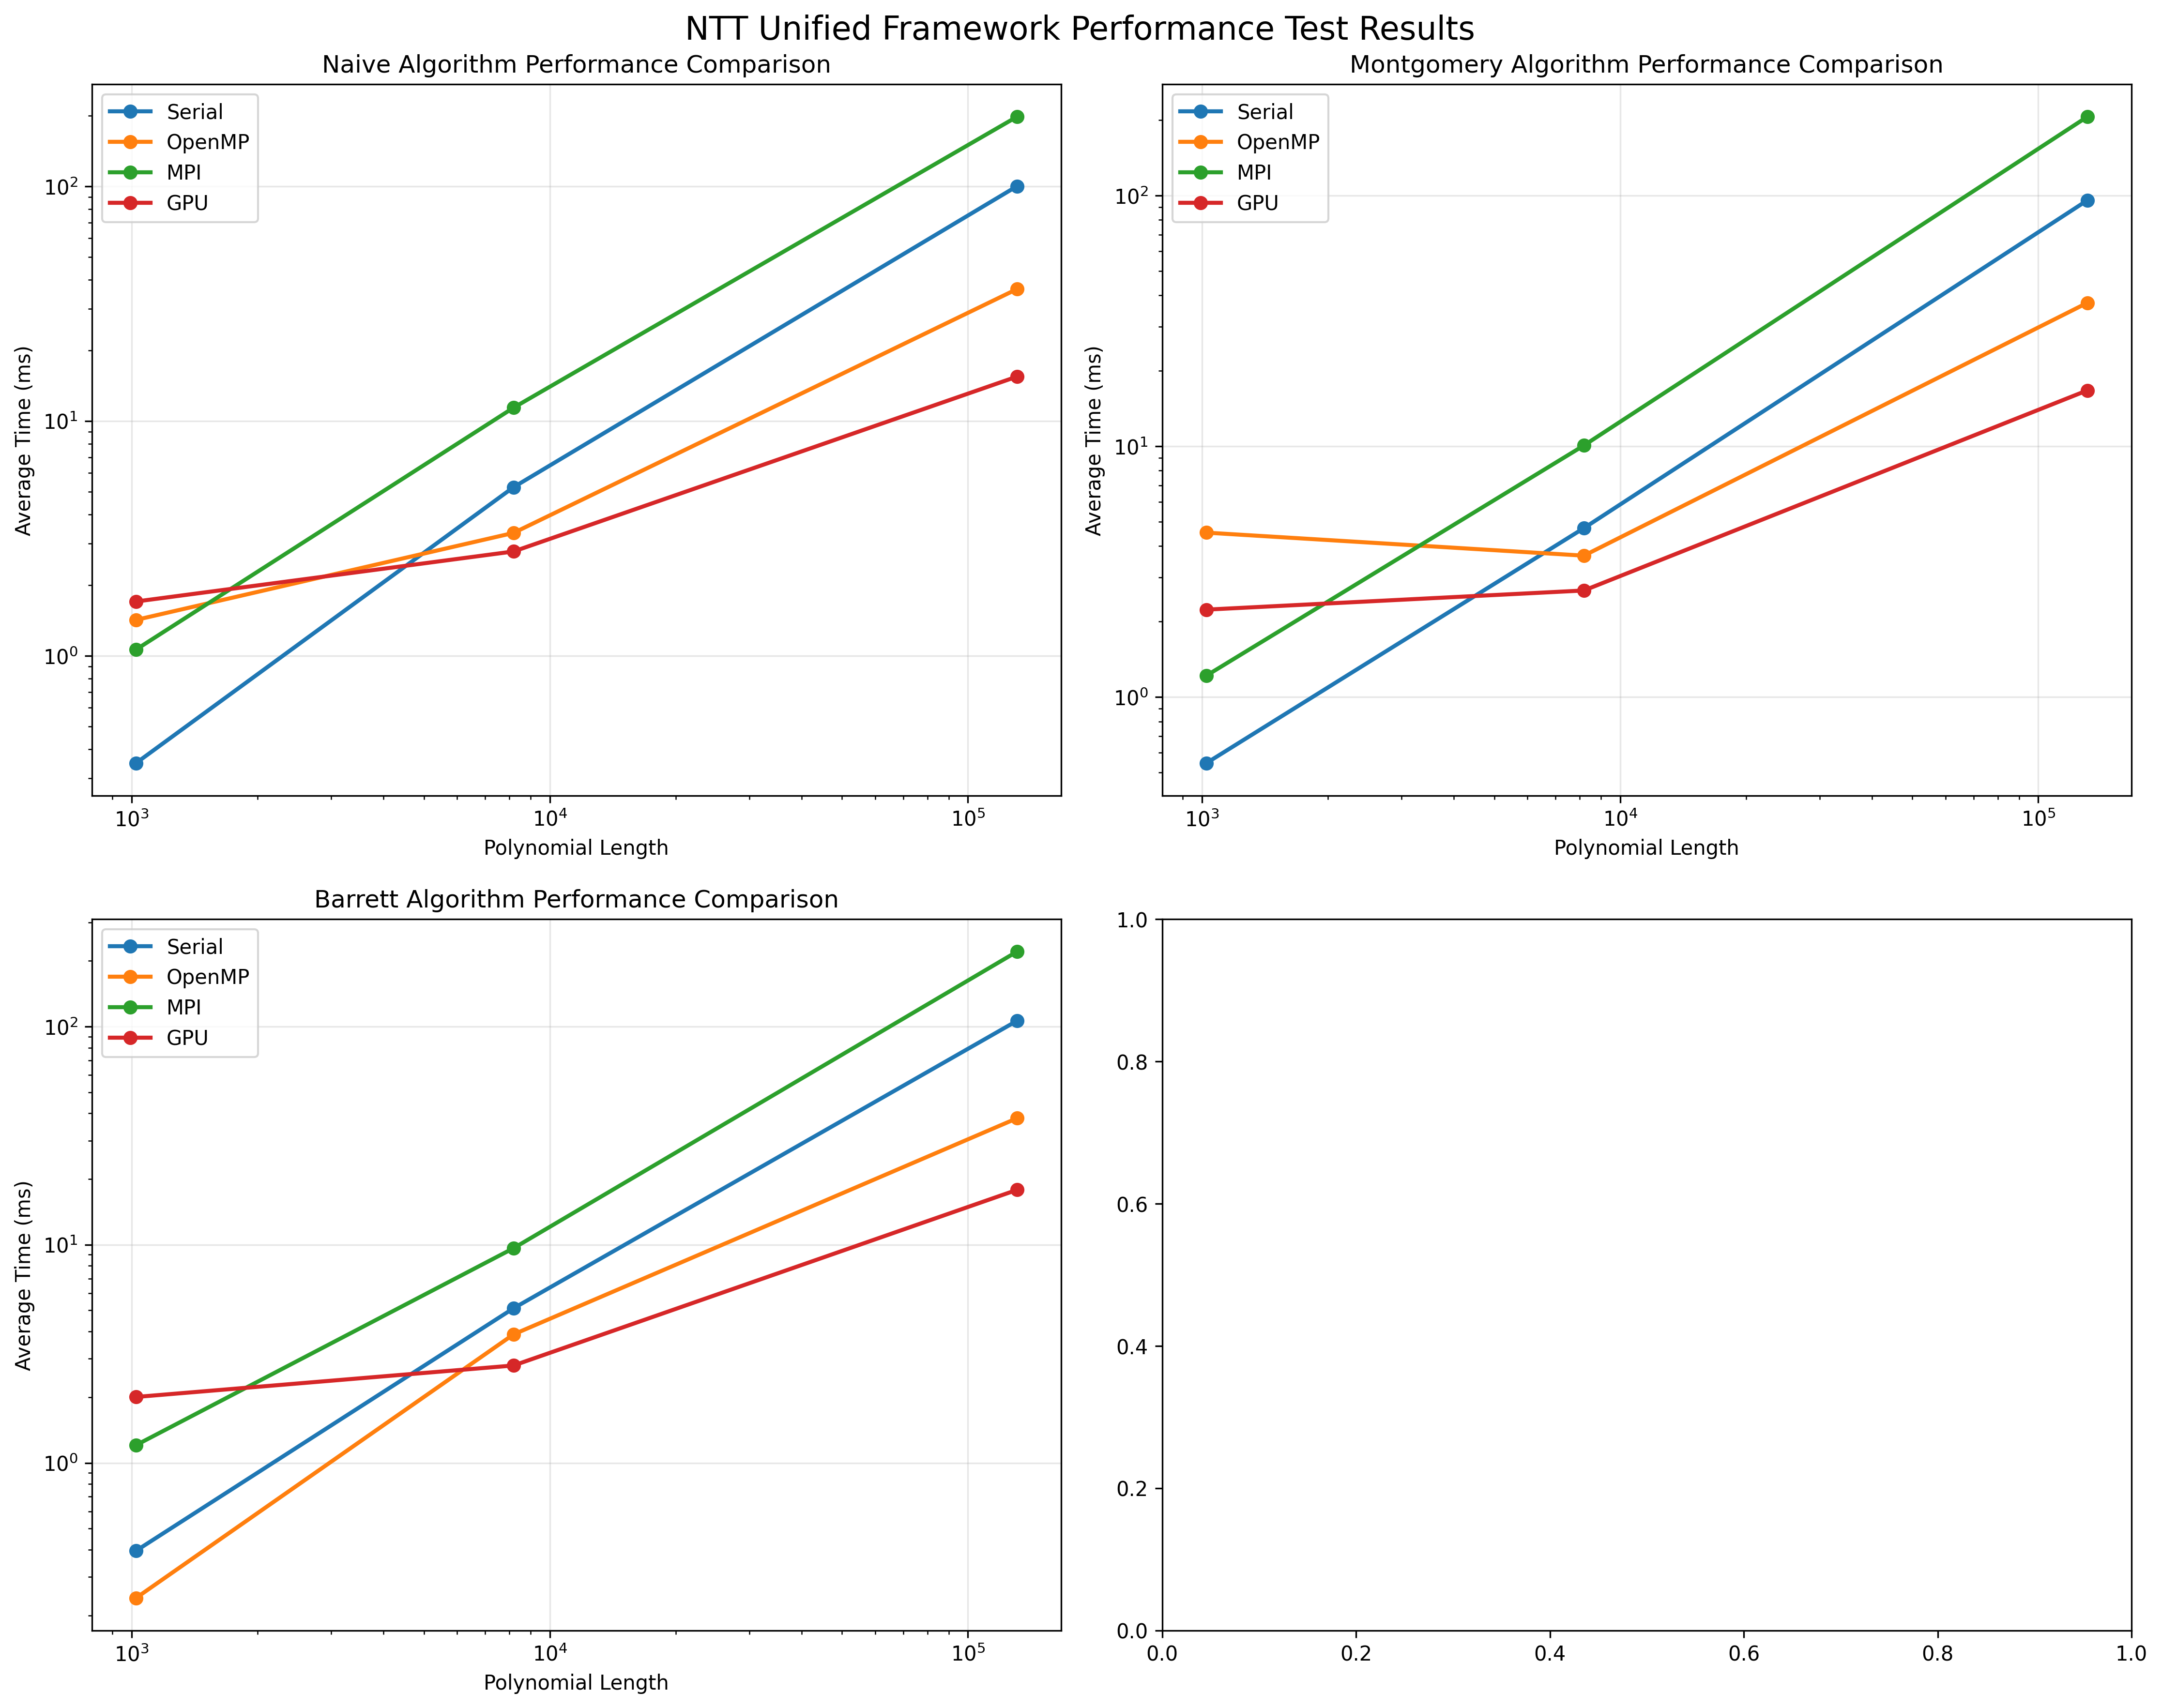
\includegraphics[width=0.8\textwidth]{performance_comparison.png}
\caption{按算法分组的性能对比}
\label{fig:performance_comparison}
\end{figure}

\paragraph{GPU并行策略} 在所有三种算法中，GPU都表现出最强的性能，尤其是在数据规模增大时，其性能优势愈发显著，最终实现了4-6倍的加速比。这得益于GPU的大规模并行计算能力，它能够将NTT中的蝶形运算分配到数千个线程上同时执行，极大地提升了计算效率。

\paragraph{OpenMP并行策略} OpenMP多线程策略在中小规模数据上表现不佳，甚至慢于串行版本，这是因为在计算量不足时，线程创建、调度和同步的开销超过了并行带来的收益。然而，当数据规模达到中等及以上（$n \ge 8192$）时，OpenMP能够实现2-3倍的稳定加速，成为CPU环境下最具性价比的并行方案。

\paragraph{串行策略} 作为性能基准，串行策略的执行时间随数据规模增大而线性增长。它是小规模数据下（$n \le 1024$）最有效的计算方式，因为此时它避免了任何并行开销。

\paragraph{MPI并行策略} 我们的MPI实现由于采用了CRT分解来创造并行位点，导致了四倍的冗余计算，因此其性能在所有规模下都远逊于其他策略。此处的MPI测试结果不应用于与其他并行策略进行性能对比，其主要价值在于展示三种模运算算法在MPI框架下的相对性能。

\subsection{按算法分析}

为了评估三种模运算算法（朴素、Montgomery、Barrett）在不同并行环境下的适应性，我们绘制了按并行策略分组的性能对比图（见图\ref{fig:strategy_grouped_comparison}）。同样需要注意，这里纵坐标代表测试平均时长，这意味着越靠下的数据点代表的性能越好。

在该图中，每张子图代表一种并行策略，图中的曲线则展示了三种模运算算法的性能差异。虽然大部分情况下三种模运算算法的性能都几乎一致，但我们还是能看出一些细微的性能区别。

\begin{figure}[htbp]
\centering
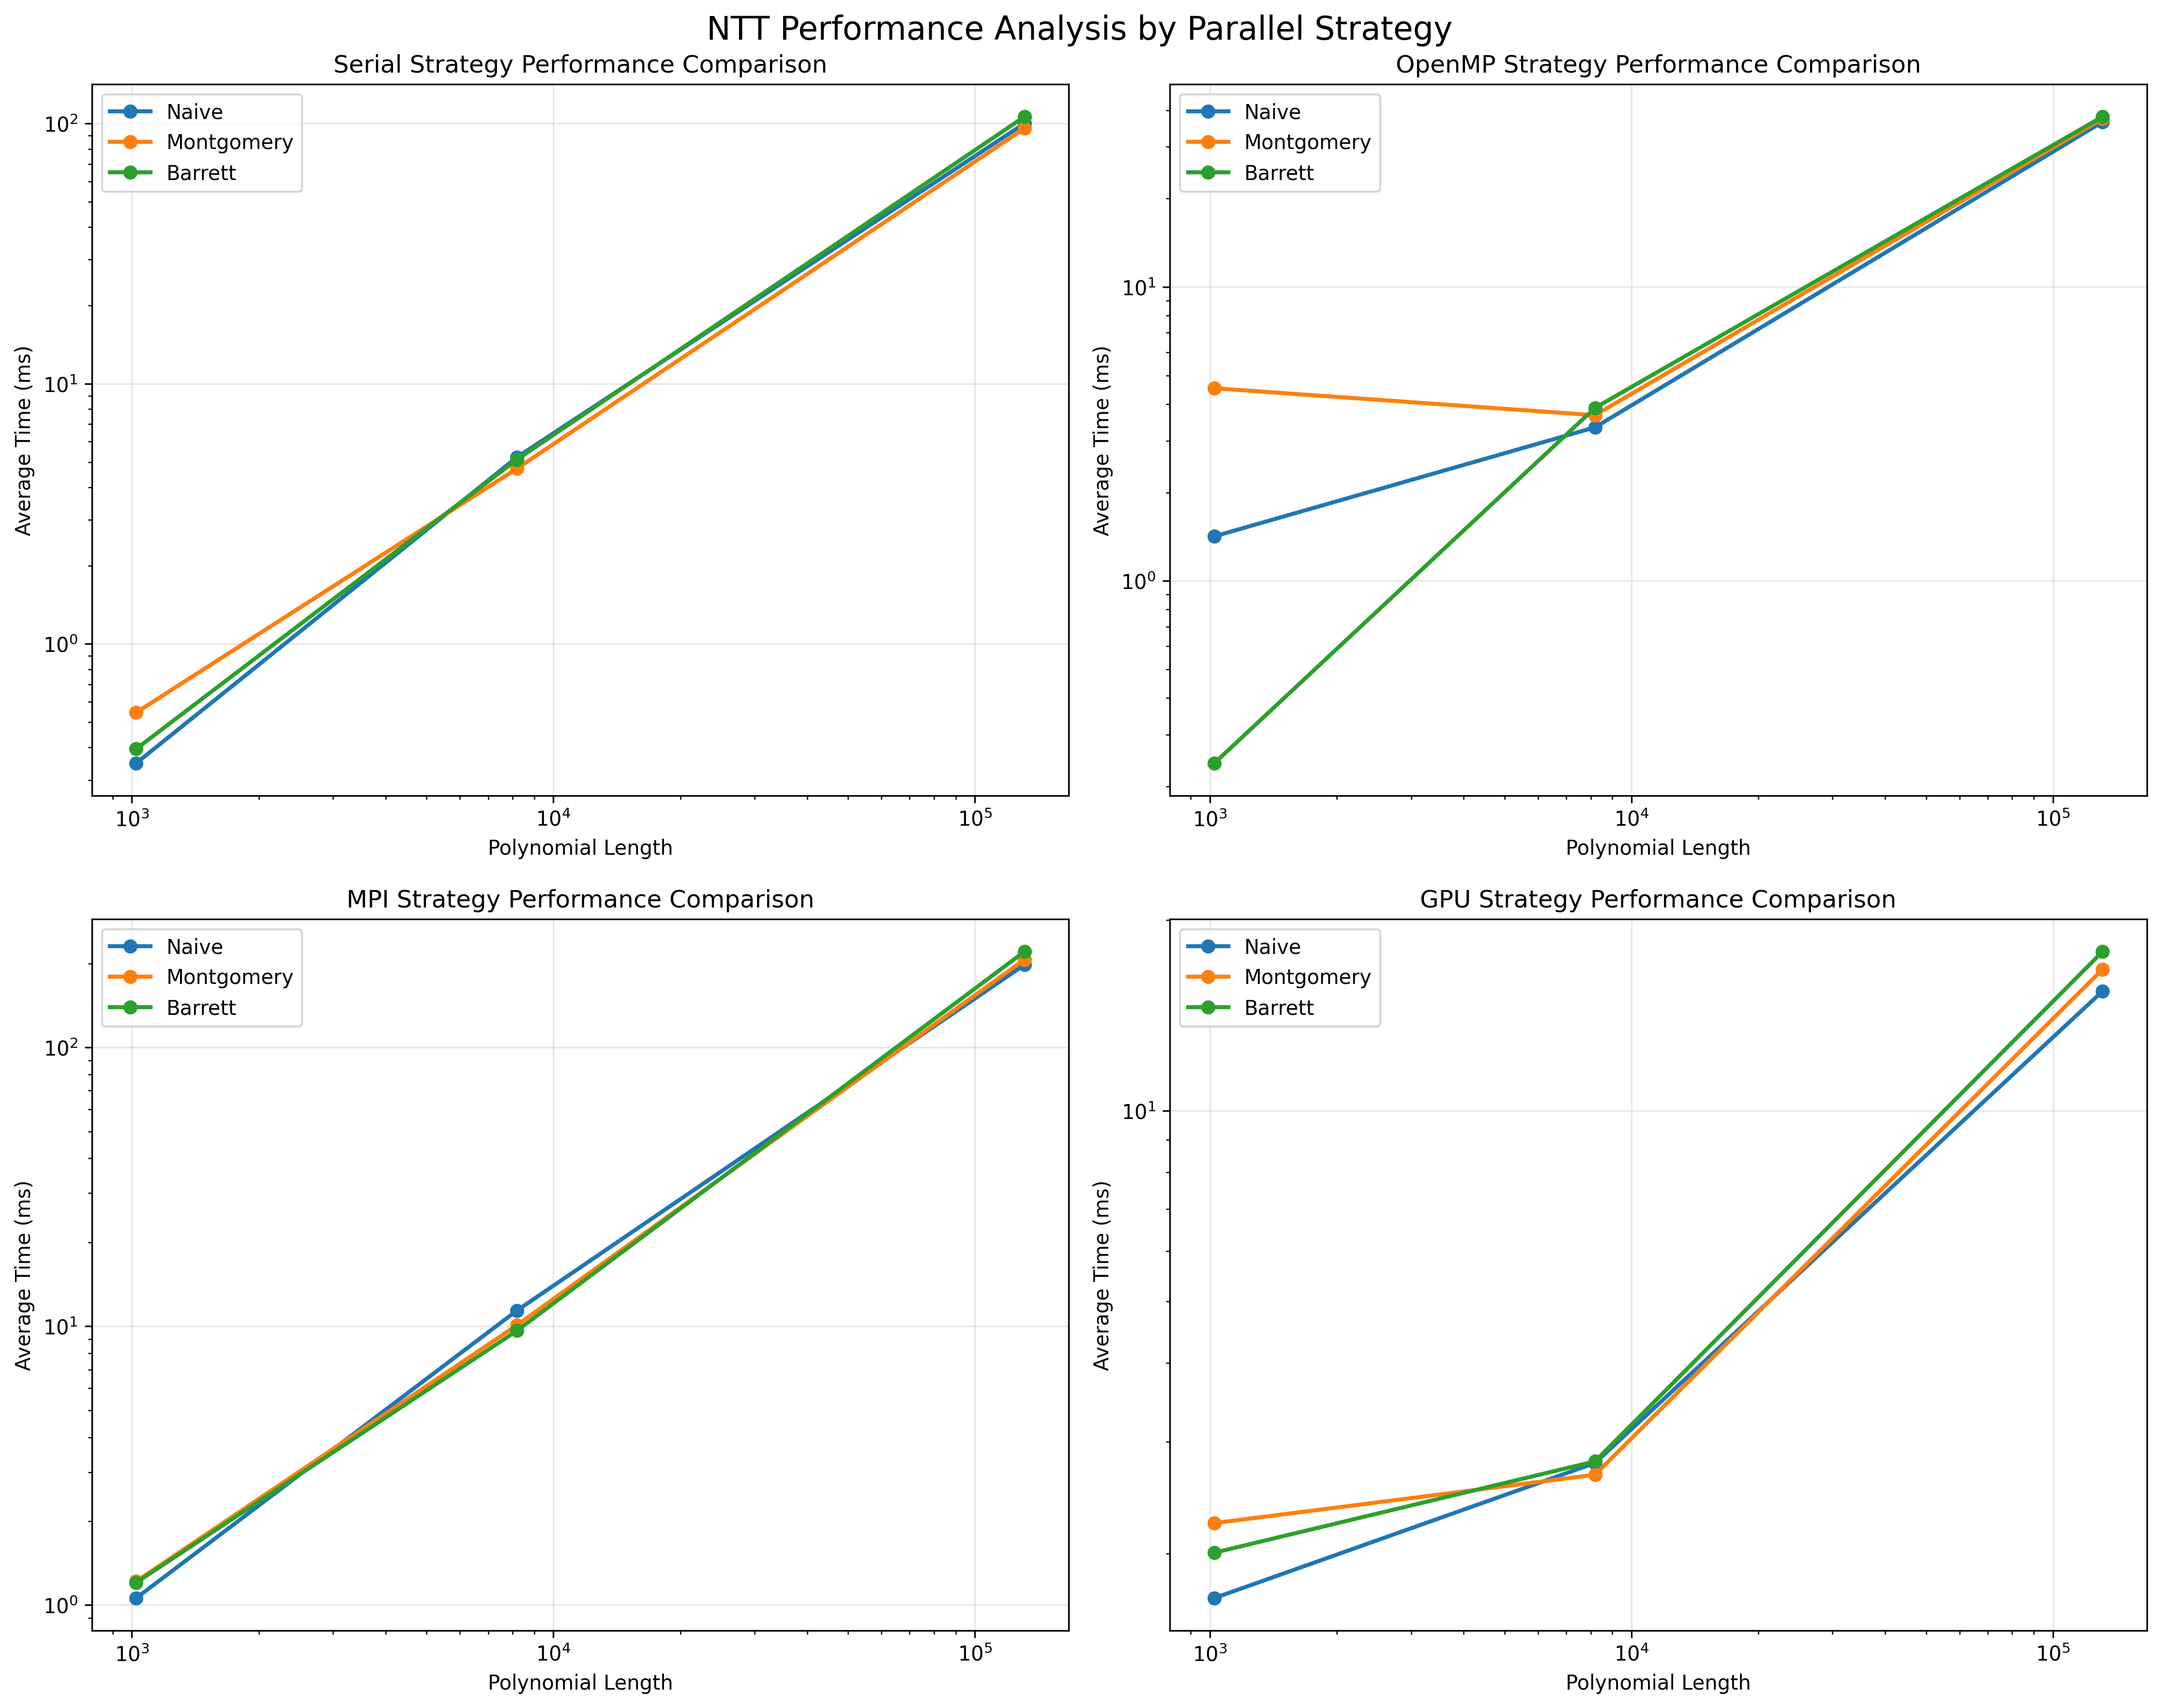
\includegraphics[width=0.8\textwidth]{strategy_grouped_comparison.png}
\caption{按并行策略分组的性能对比}
\label{fig:strategy_grouped_comparison}
\end{figure}

\paragraph{串行环境下的算法对比} 在串行模式下，Montgomery算法的性能最优，Barrett次之，朴素算法最慢。这完全符合理论预期：Montgomery通过将昂贵的模运算转化为高效的位运算和加法，显著提升了计算效率。

\paragraph{OpenMP环境下的算法对比} 在OpenMP多线程环境下，Barrett算法在小规模数据上表现出惊人的性能，甚至超越了其他所有组合。但随着规模增大，三种算法的性能差距逐渐缩小，最终趋于一致。

\paragraph{GPU环境下的算法对比} 在GPU大规模并行环境下，三种算法的性能差异被进一步缩小。这表明GPU的强大计算能力可以有效"掩盖"底层模运算实现的微小差异，无论是哪种算法，只要能够被拆解为足够多的细粒度任务，都能在GPU上获得极高的并行效率。

\paragraph{SIMD指令级并行分析} 由于测试环境限制，我们未能直接进行SIMD性能测试。但根据第二次实验（SIMD并行化实验）的实验结果，基于ARM NEON的SIMD优化能在Montgomery算法上取得2-4倍的性能提升。SIMD与Montgomery的良好结合，是因为后者将运算分解为SIMD指令集能够高效处理的基础位运算和整数运算。

\subsection{按数据规模分析与工程建议}

综合以上所有分析，我们可以根据数据规模为不同的应用场景提供具体的工程实现建议。

\paragraph{小规模数据 ($n \le 1024$)} 在此规模下，并行化带来的开销（如线程创建、数据传输）往往超过其收益。因此，\textbf{串行算法是最佳选择}。在三种串行算法中，Montgomery和Barrett算法性能接近且表现最优。因此，推荐使用\textbf{串行Montgomery或Barrett算法}。

\paragraph{中等规模数据 ($1024 < n \le 8192$)} 当数据规模增大到中等水平时，多线程并行的优势开始显现。测试结果表明，\textbf{OpenMP并行化}在这一区间内能够提供最佳的性能。其中，\textbf{OpenMP与Barrett算法的组合}表现最为出色。

\paragraph{大规模数据 ($n > 8192$)} 对于大规模数据，GPU的强大并行计算能力使其成为无可争议的最优选择。此时，底层模运算算法的差异已不再是主要矛盾。\textbf{任何一种模运算算法与GPU的结合}都能取得最佳性能。在我们的测试中，\textbf{朴素算法+GPU}的组合取得了最高的6.5倍加速比。

\paragraph{总结}
综合以上分析，我们认为，在实际应用中，可以构建一个动态调度系统——在任务开始前，首先判断输入数据规模$n$：若$n \le 1024$，则调用串行Montgomery实现；若$1024 < n \le 8192$，则调用OpenMP-Barrett实现；若$n > 8192$，则调用GPU实现。这样的动态选择策略能够确保在任何数据规模下都能获得接近最优的计算性能。对于MPI，除非应用场景是处理u64等超大数据类型且必须使用CRT分解，否则在当前u32场景下不推荐使用我们现有的MPI实现。

\section{尾声}

回顾整个 NT​T 并行优化系列实验，我们历时一个学期，先后完成了 SIMD 指令级并行（Lab2）、多线程并行（Lab3）、多进程分布式并行（Lab4）、GPU 极细粒度并行（Lab5）以及最后的统一框架与全面性能测试。一路走来，我们既经历了"写出来能跑"的朴素喜悦，也经历了在缓存失效、线程争用与通信瓶颈面前的挫败，更在一次次 profiler 的火焰图与显存带宽的红线里收获了洞见。

\paragraph{SIMD 实验的收获与遗憾} 在 Lab2 中，我们第一次将 NTT 的蝶形循环拆解为向量化友好的形态，尝试使用 ARM NEON 指令集实现四路并行的 Montgomery 模运算。通过重构数据布局、预计算常量、手写汇编级 intrinsic，我们让性能提升了三个数量级，也第一次体会到"把数学写进寄存器"的快感。然而，由于实验服务器并不支持 NEON，最终的性能只能通过离线跑分间接验证，这成为本系列实验最早的遗憾：缺乏真正的硬件环境，很难进一步探索更深层的 SIMD 优化，例如混合基 NT​T 与向量内分段卷积。

\paragraph{多线程实验的收获与遗憾} Lab3 让我们直面 CPU 多核并行的工程细节。从最简单的 `#pragma omp parallel for` 开始，我们学会了用数据依赖和任务粒度来定位并行位点；当 OpenMP 在小规模问题上出现反加速时，我们又实现了线程池，体会到如何用条件变量与原子计数来平衡开销与吞吐。这一阶段最大的收获是建立了"串行代码 \rightarrow 便于并行化的重构 \rightarrow 并行代码"的范式。但也正是在这一阶段，我们第一次感受到内存带宽的天花板：四个物理核心在 8 线程以后几乎不再加速，说明计算已经从算术密集型转向了带宽受限型。若能更早地引入 cache blocking 或 NUMA 亲和性，也许可以再挖掘一部分潜力。

\paragraph{MPI 实验的收获与遗憾} Lab4 将战场从共享内存搬到了分布式内存。为了让 MPI 在 u32 环境下"有事可做"，我们使用了中国剩余定理把同一段计算复制了四遍——这在功能上可行，却把理论上的四进程加速变成了四倍计算量。我们学到了 Rank、Communicator 与 Bcast/Reduce 的用法，也在调试挂死与死锁中学会了把 `mpirun -np` 写成脚本参数。遗憾的是，由于实验硬件仍局限在单机多核，网络通信被系统调用虚拟化，性能不仅没有提升，反而因冗余计算而雪崩。这段经历提醒我们：并行并不等于复制计算，算法与架构要协同设计。

\paragraph{GPU 实验的收获与遗憾} Lab5 是整个系列的高潮。我们把三层循环展平成"一线程一蝶形"，用预计算旋转因子消除了循环携带依赖，再用共享内存消化数据复用，第一次让十几万 thread 在同一个 kernel 中并肩作战。性能从毫秒量级跌入微秒量级，也让我们真正体会到"算子融合""访存对齐""Occupancy"这些 CUDA 关键词背后的含义。遗憾同样存在：线程块内同步仍依赖 `__syncthreads()` 全栅栏，导致 warp 内指令级并行度没有完全榨干；若有时间继续探索 Shuffle 指令或 Tensor Core 上的 INT32 Tensor MMA，也许还能再减少一次全局访存。

\paragraph{统一框架与测试的反思} 最终的统一框架把三种模运算与四种并行策略装进同一个函数接口，从"写得对"走向了"写得像产品"。这一过程中，我们第一次处理宏配置冲突、跨平台 CMake、统一随机测试与持续集成，也第一次用 PGFPlots 画图批量生成报告。真正运行大规模测试时，我们才发现：最耗时的不是计算，而是把所有结果汇总、对齐、可视化——这让我们意识到工程化的重要性。

\paragraph{方法论的沉淀} 贯穿所有实验，我们逐步形成了三条方法论：第一，任何并行优化都必须先做依赖分析，用可视化手段（火焰图、Roofline、Nsight）定位瓶颈；第二，先用"小步快跑"的原型验证正确性，再用"自下而上"的层次优化榨干性能；第三，把"可维护性"当作一等公民，用模板、线程池、RAII 和条件编译让代码在扩展时不崩溃。

\paragraph{未来展望} 如果时间与资源允许，我们希望继续探索三个方向：其一，引入混合基（radix-​4/8）NTT 与自适应线程映射，进一步提升 GPU 的存算比；其二，实现真正分布式的 u64 CRT + MPI，在多节点 GPU 集群上验证横向扩展性；其三，使用 Tuning Framework（如 TVM MetaSchedule）做参数自动搜索，让线程块大小、寄存器分配和流水线深度由数据驱动而非经验决定。

短暂的一个学期无法穷尽 NTT 优化的全部可能，但从第一次把蝶形运算写成循环，到今天能在 GPU 上跑到微秒级延迟，我们已经完成了从"写对"到"写快"再到"写稳"的渐进旅程。实验会结束，但分析依旧、改进亦然。愿这些代码片段、火焰图和性能曲线，能成为下一次优化的起点，也为同态加密与高性能计算的交汇贡献一砖一瓦。

\end{document}